\documentclass[12pt]{article}
\usepackage[utf8]{inputenc}
\usepackage{graphicx} % Allows you to insert figures
\usepackage{amsmath} % Allows you to do equations
\usepackage{fancyhdr} % Formats the header
\usepackage{geometry} % Formats the paper size, orientation, and margins
\usepackage[style=authoryear-ibid,backend=biber]{biblatex} % Allows you to do citations - does Harvard style and compatible with Zotero
\addbibresource{Example.bib} % Tells LaTeX where the citations are coming from. This is imported from Zotero
\usepackage[english]{babel}
\usepackage{csquotes}
\usepackage{background}
\usepackage{minted}
\renewcommand*{\nameyeardelim}{\addcomma\space} % Adds comma in in-text citations
\linespread{1.5} % About 1.5 spacing in Word
\setlength{\parindent}{0pt} % No paragraph indents
\setlength{\parskip}{1em} % Paragraphs separated by one line
\renewcommand{\headrulewidth}{0pt} % Removes line in header
\geometry{a4paper, portrait, margin=1in}
\setlength{\headheight}{14.49998pt}
\backgroundsetup{scale=1,angle=0,opacity=0.175,contents={
\includegraphics[scale=0.25]{1200px-Vellore_Institute_of_Technology_seal_2017.png}}}


\begin{document}
\begin{titlepage}
\NoBgThispage
   \begin{center}
        \begin{figure}[h] % h - Place the float here, i.e., approximately at the same point it occurs in the source text (however, not exactly at the spot)
        \centering
        
\includegraphics[width=15cm]{1583124354phpJTtnK5.png}
        \end{figure}

        \Huge{Digital Assignment 4}

        \vspace{0.5cm}
        \LARGE{20BIT0406 - Sanchit Sandeep Khedkar}
       
        \vspace{2.5 cm}
        \Large{2022-04-04}
        
        \vspace{0.25 cm}
        \Large{ITE3001 - Data Communication and Computer Networks}
        \large{VL2021220500483 L33+L34}
       

       \vfill
    \end{center}
\end{titlepage}
\newpage

\setcounter{page}{2}
\pagestyle{fancy}
\fancyhf{}
\rhead{\thepage}

Q1.  
Write a UDP client server program to find out the beginning address of the block if the address 134.67.100.1/22 is sent by the client to the server. Then, the server will send the first address back to the client.

Ans- \\ Code- \\ udpBeginningAddrServer.py-\inputminted{python}{udpBeginningAddrServer.py}
udpBeginningAddrClient.py- \inputminted{python}{udpBeginningAddrClient.py}
\newpage
Output-
\begin{figure}[h] % h - Place the float here, i.e., approximately at the same point it occurs in the source text (however, not exactly at the spot)
\centering
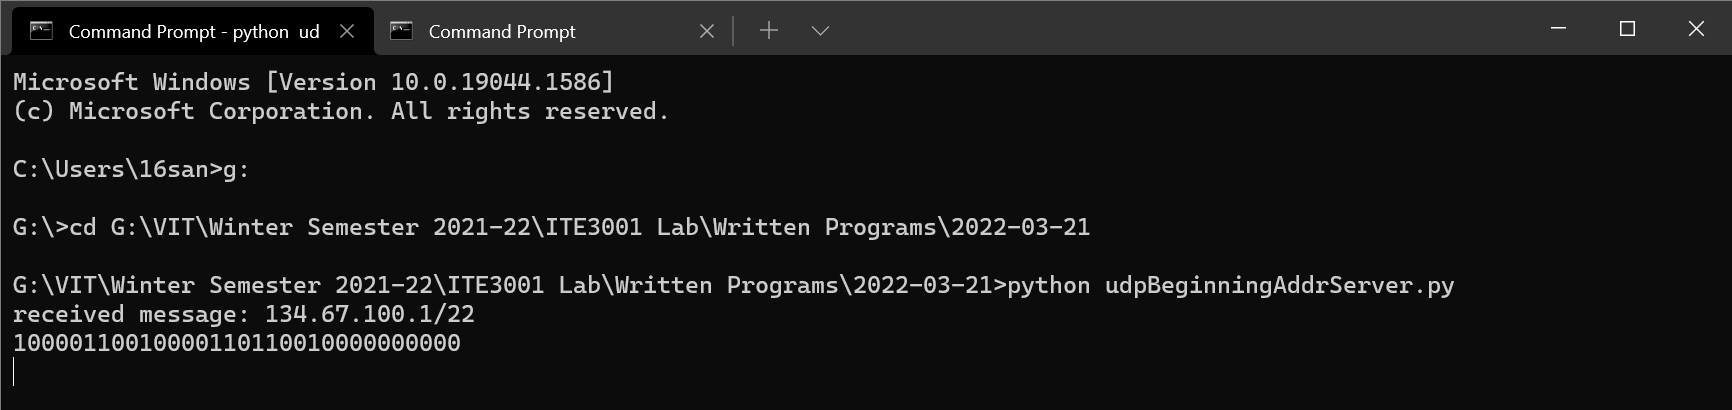
\includegraphics[width=\textwidth]{udpBeginningAddrServer.py.png}
\caption{Server output}
\end{figure}
\begin{figure}[h] % h - Place the float here, i.e., approximately at the same point it occurs in the source text (however, not exactly at the spot)
\centering
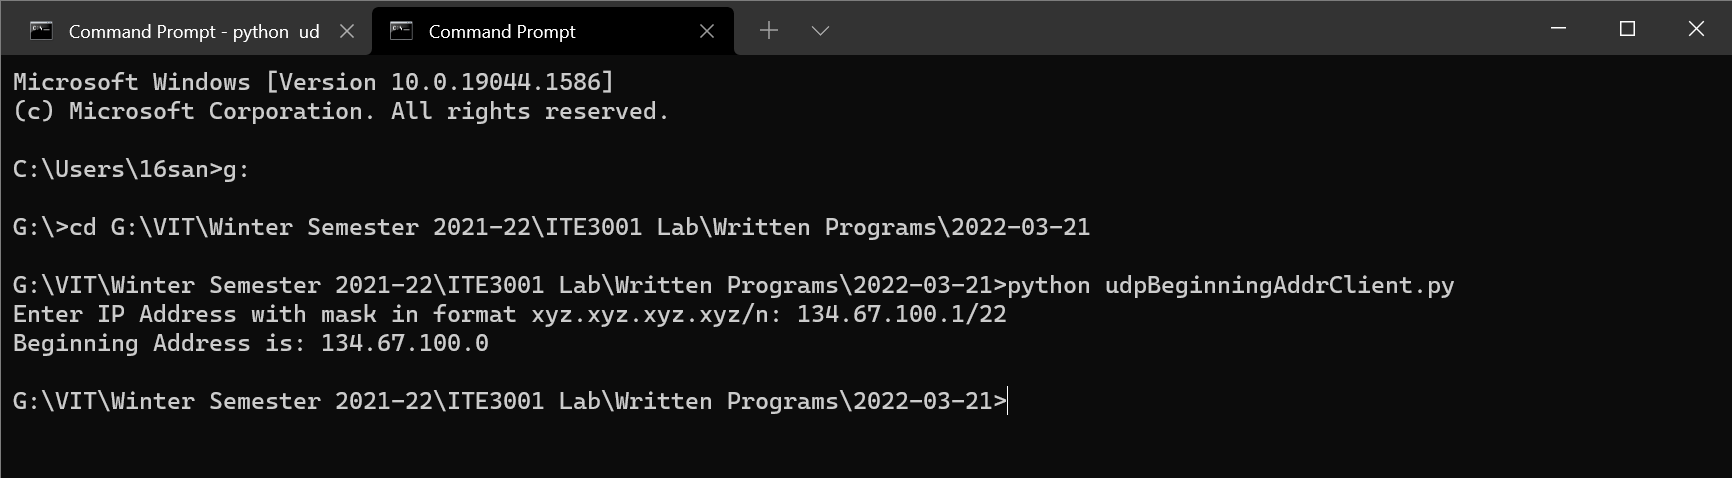
\includegraphics[width=\textwidth]{udpBeginningAddrClient.py.png}
\caption{Client output}
\end{figure}
\newpage

Q2. Implement a UDP socket for the design of subnets. The client will send 151.45.0.0/24 to the server. The sever will create 8 subnets and sends the first and last address of each subnet to the client. Finally, the client will print the range of addresses of each subnet.
\newline
Ans- \\ Code- \\ udpSubnetServer.py-\inputminted{python}{udpSubnetServer.py}
udpSubnetClient.py- \inputminted{python}{udpSubnetClient.py}
Output-
\begin{figure}[h] % h - Place the float here, i.e., approximately at the same point it occurs in the source text (however, not exactly at the spot)
\centering
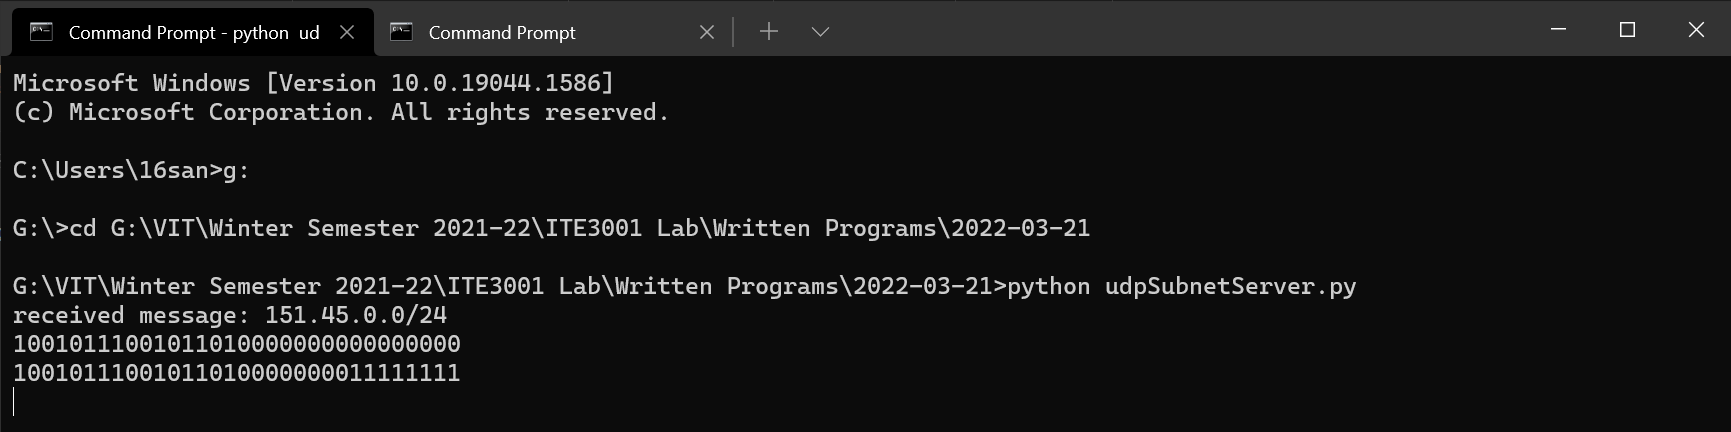
\includegraphics[width=\textwidth]{udpSubnetServer.py.png}
\caption{Server output}
\end{figure}
\begin{figure}[h] % h - Place the float here, i.e., approximately at the same point it occurs in the source text (however, not exactly at the spot)
\centering
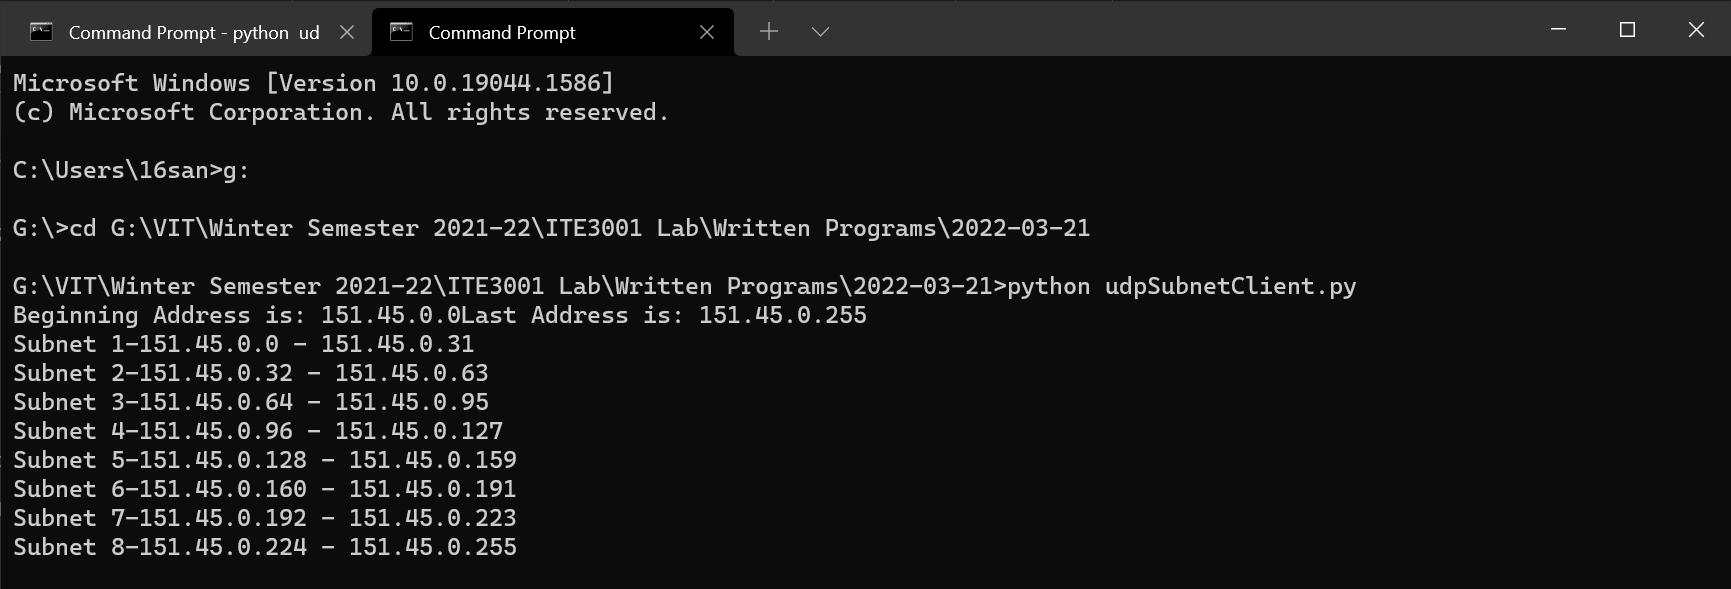
\includegraphics[width=\textwidth]{udpSubnetClient.py.png}
\caption{Client output}
\end{figure}
\newpage
\newpage
Q3.Create different topologies using the cisco packet tracer. Show the simulation output of all the topologies as a snapshot.
Output-
\begin{figure}[h] % h - Place the float here, i.e., approximately at the same point it occurs in the source text (however, not exactly at the spot)
\centering
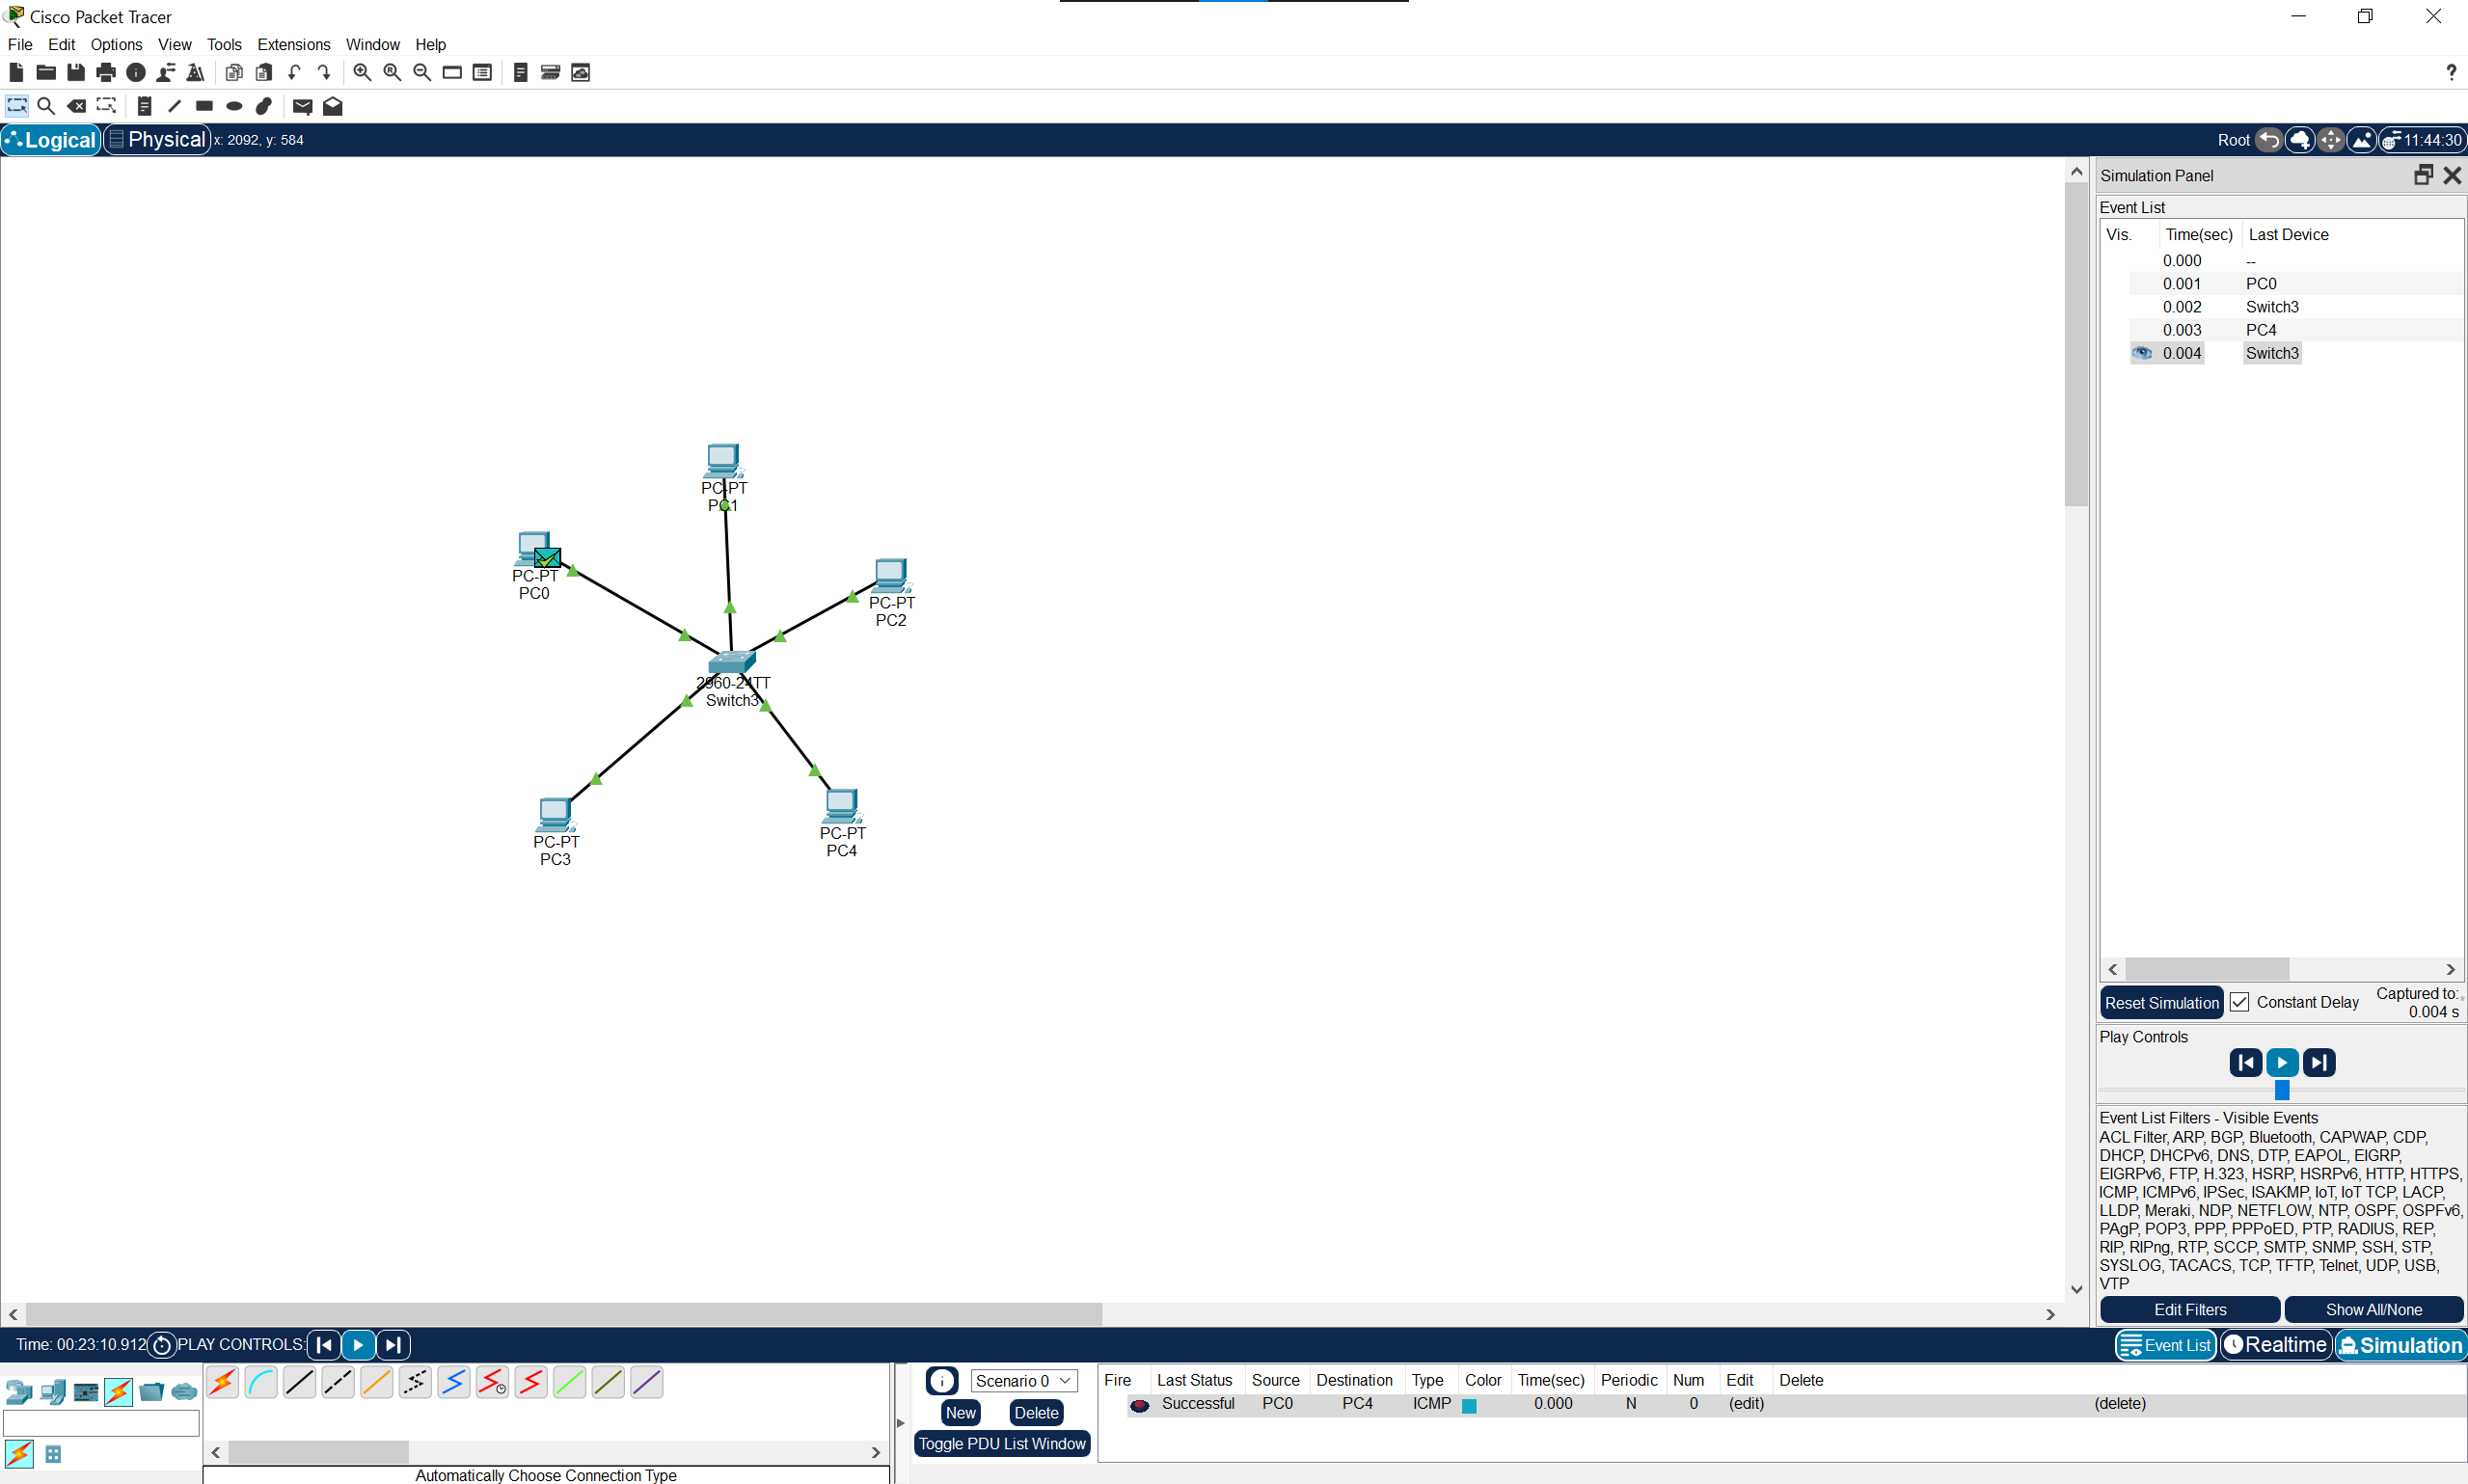
\includegraphics[width=\textwidth]{star.png}
\caption{Star topology}
\end{figure}
\begin{figure}[h] % h - Place the float here, i.e., approximately at the same point it occurs in the source text (however, not exactly at the spot)
\centering
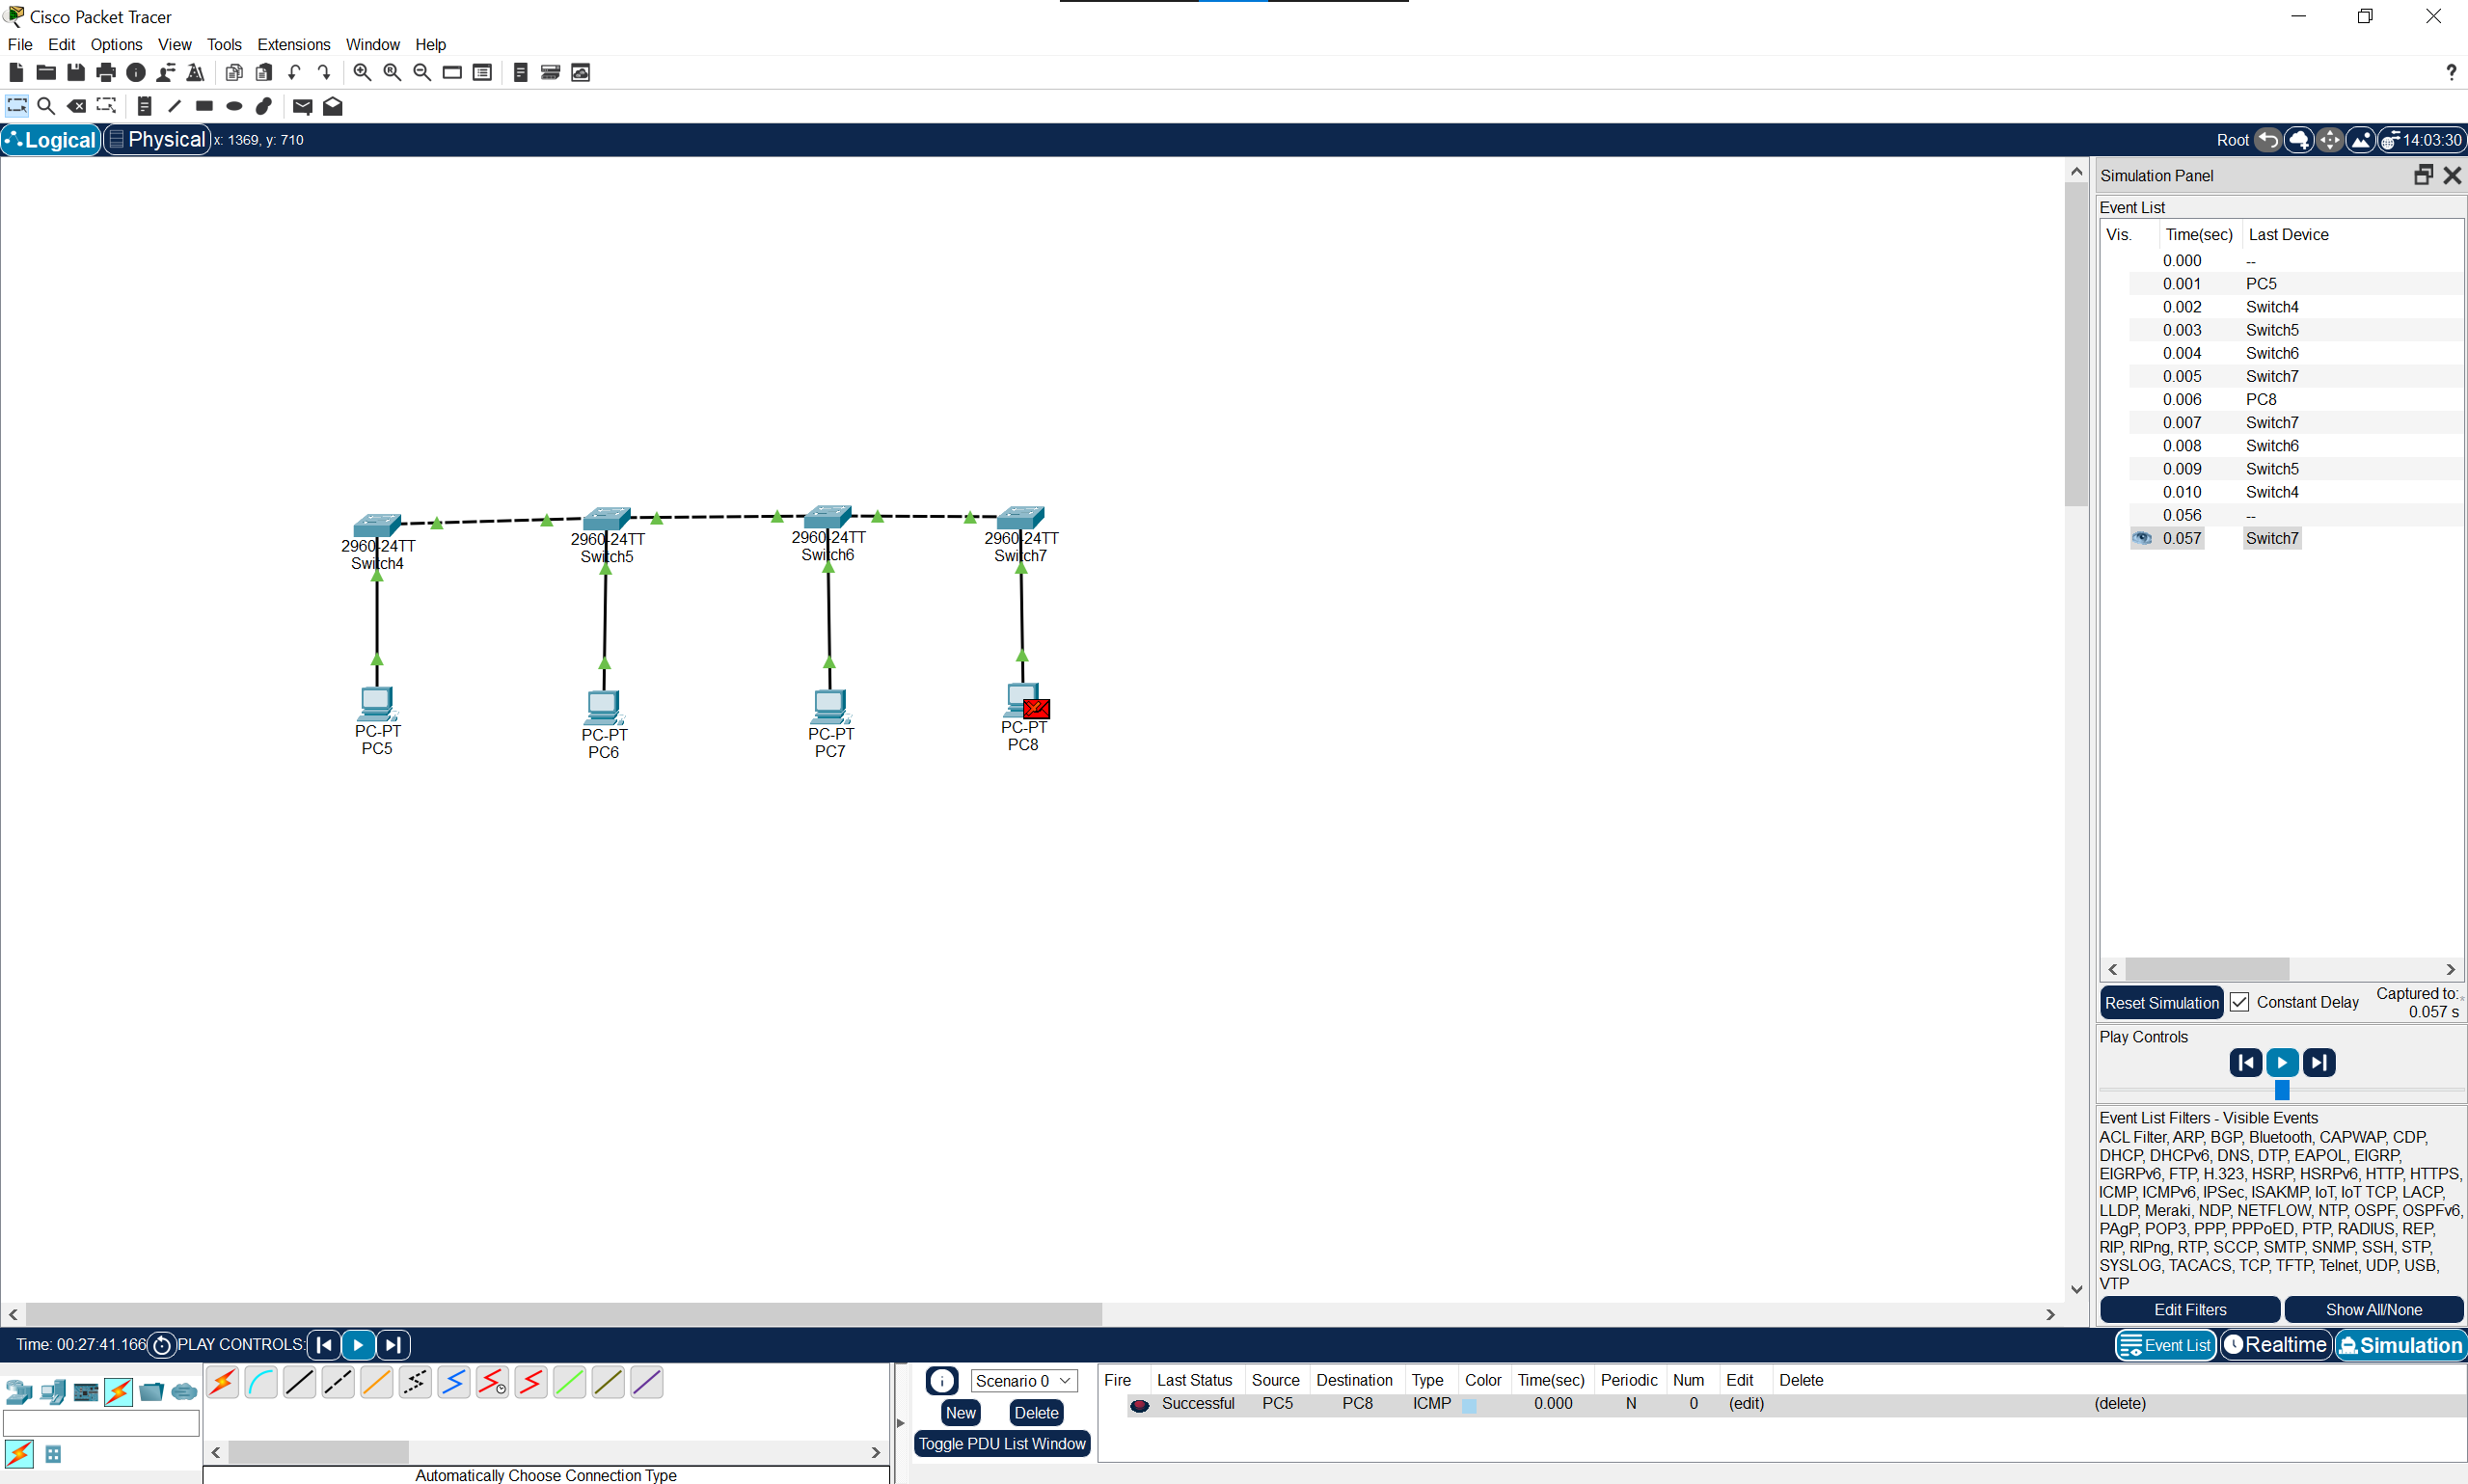
\includegraphics[width=\textwidth]{bus.png}
\caption{Bus topology}
\end{figure}
\begin{figure}[h] % h - Place the float here, i.e., approximately at the same point it occurs in the source text (however, not exactly at the spot)
\centering
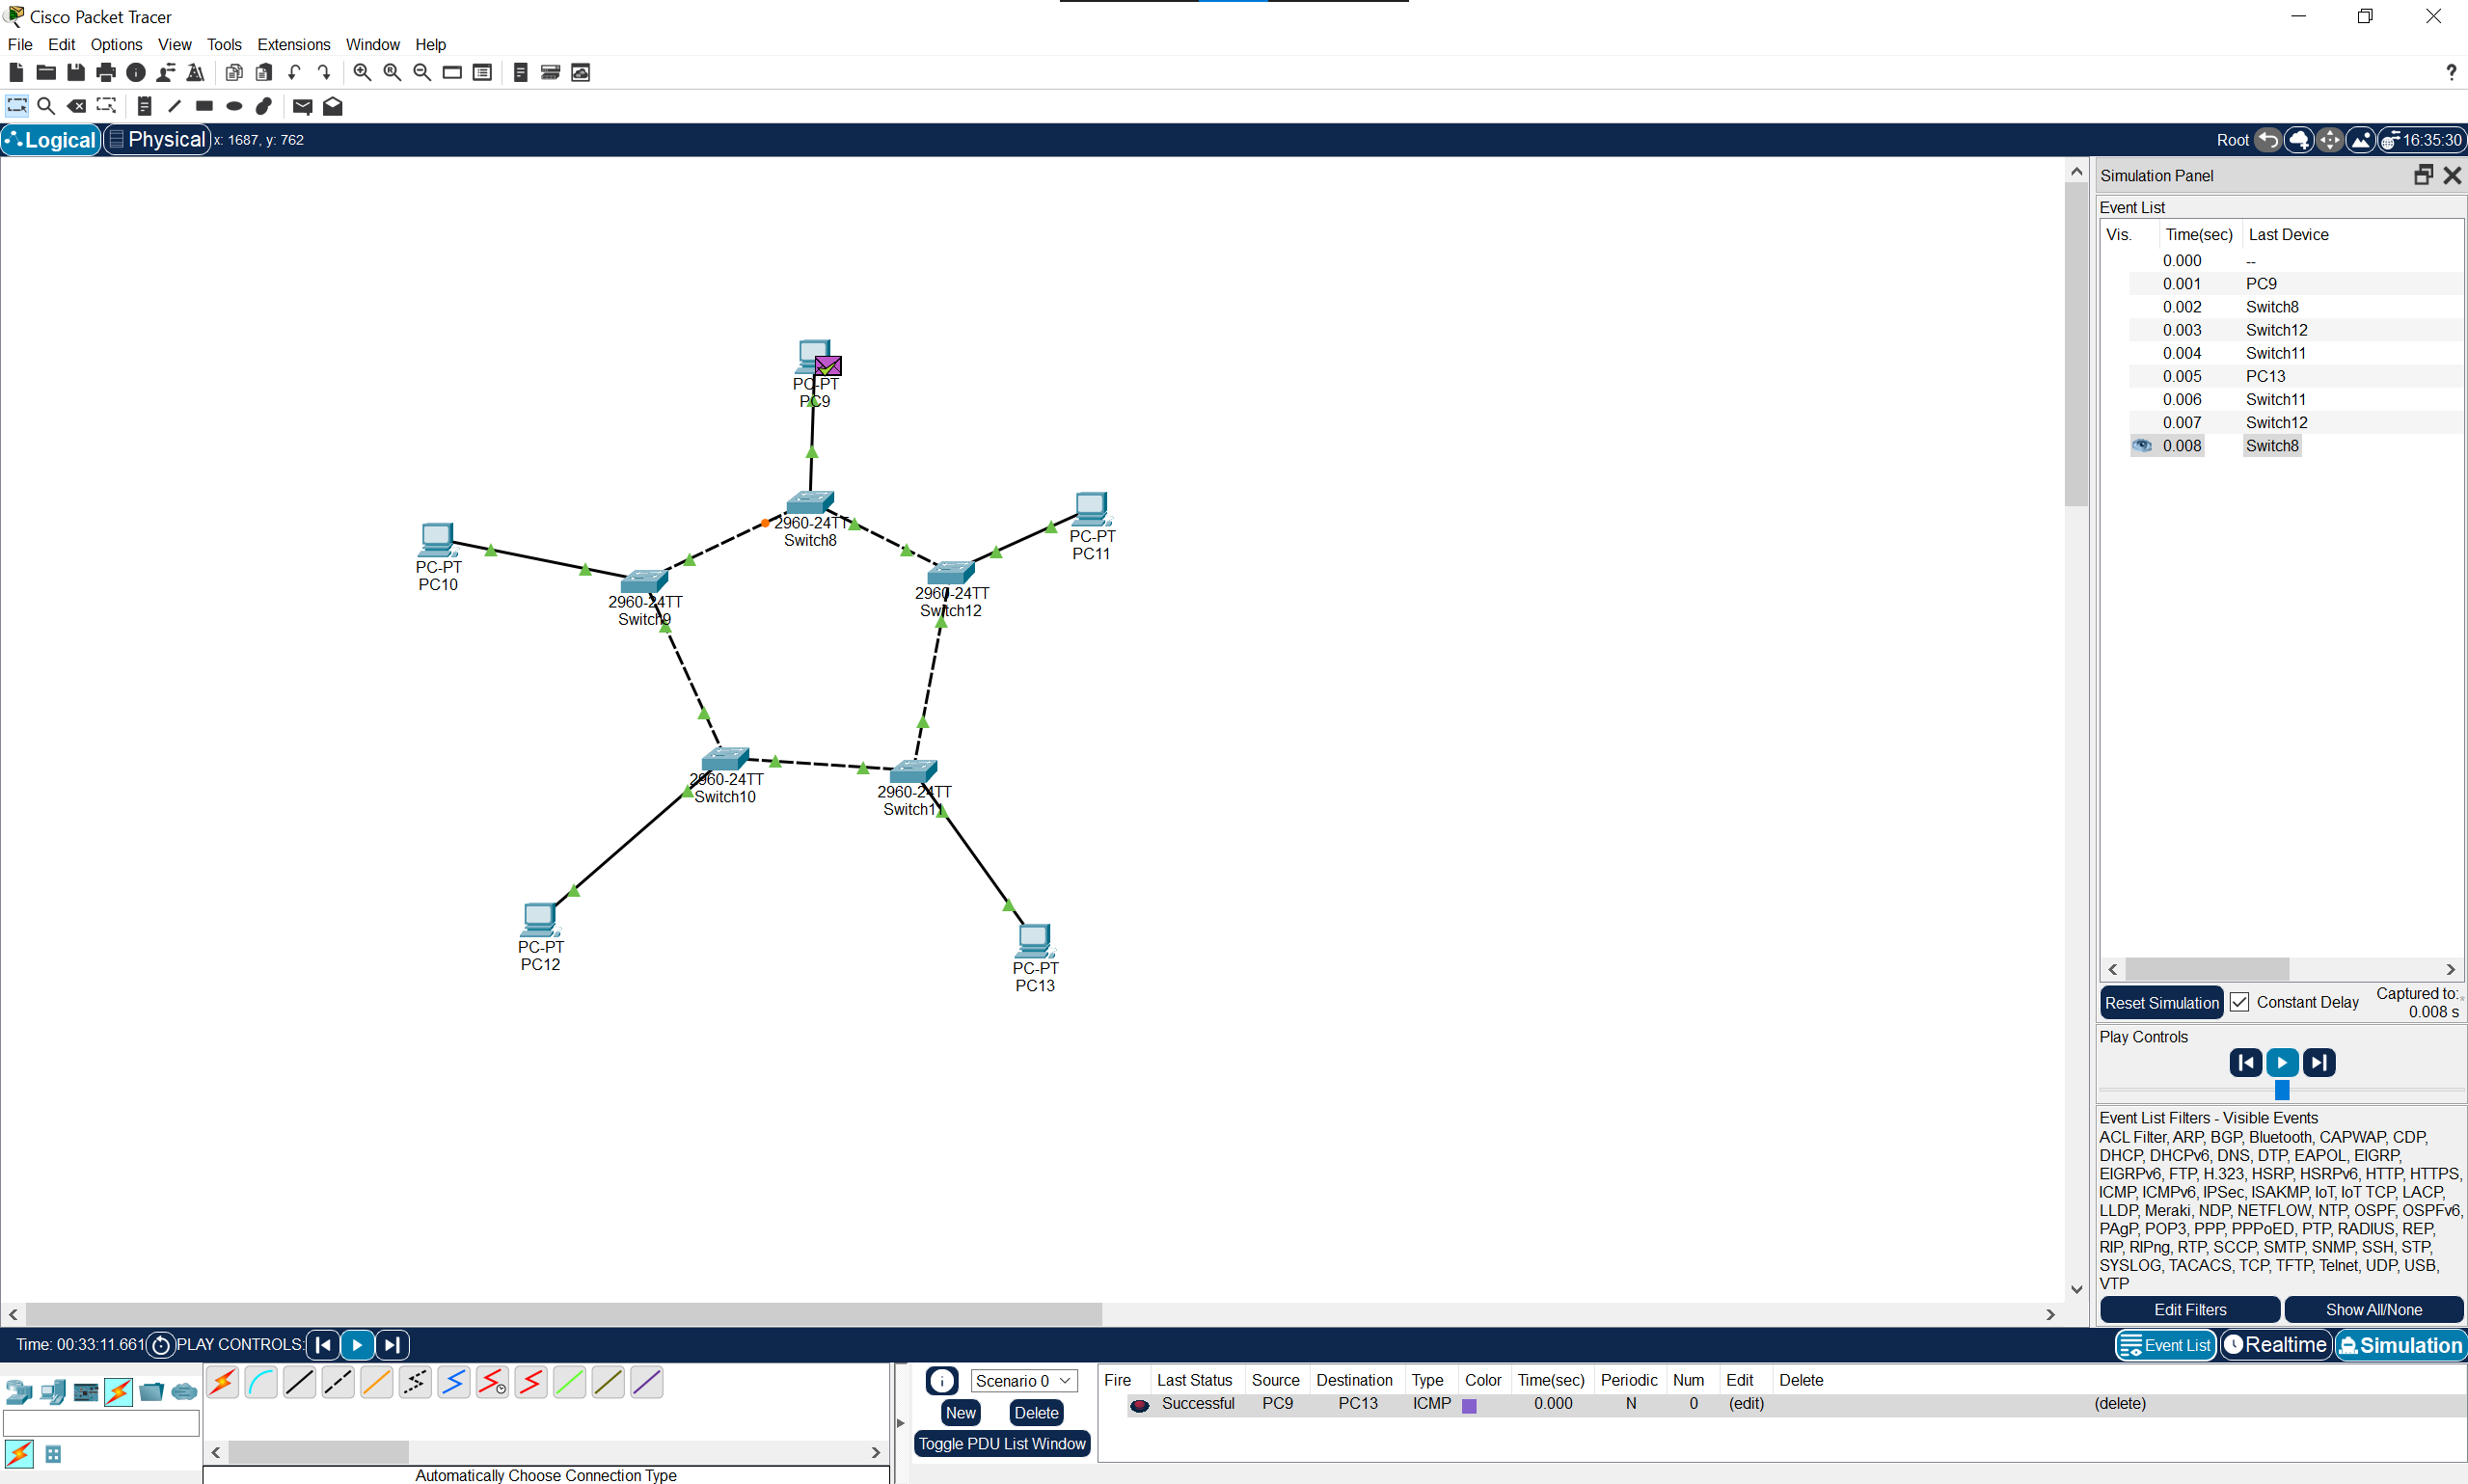
\includegraphics[width=\textwidth]{ring.png}
\caption{Ring topology}
\end{figure}
\begin{figure}[h] % h - Place the float here, i.e., approximately at the same point it occurs in the source text (however, not exactly at the spot)
\centering
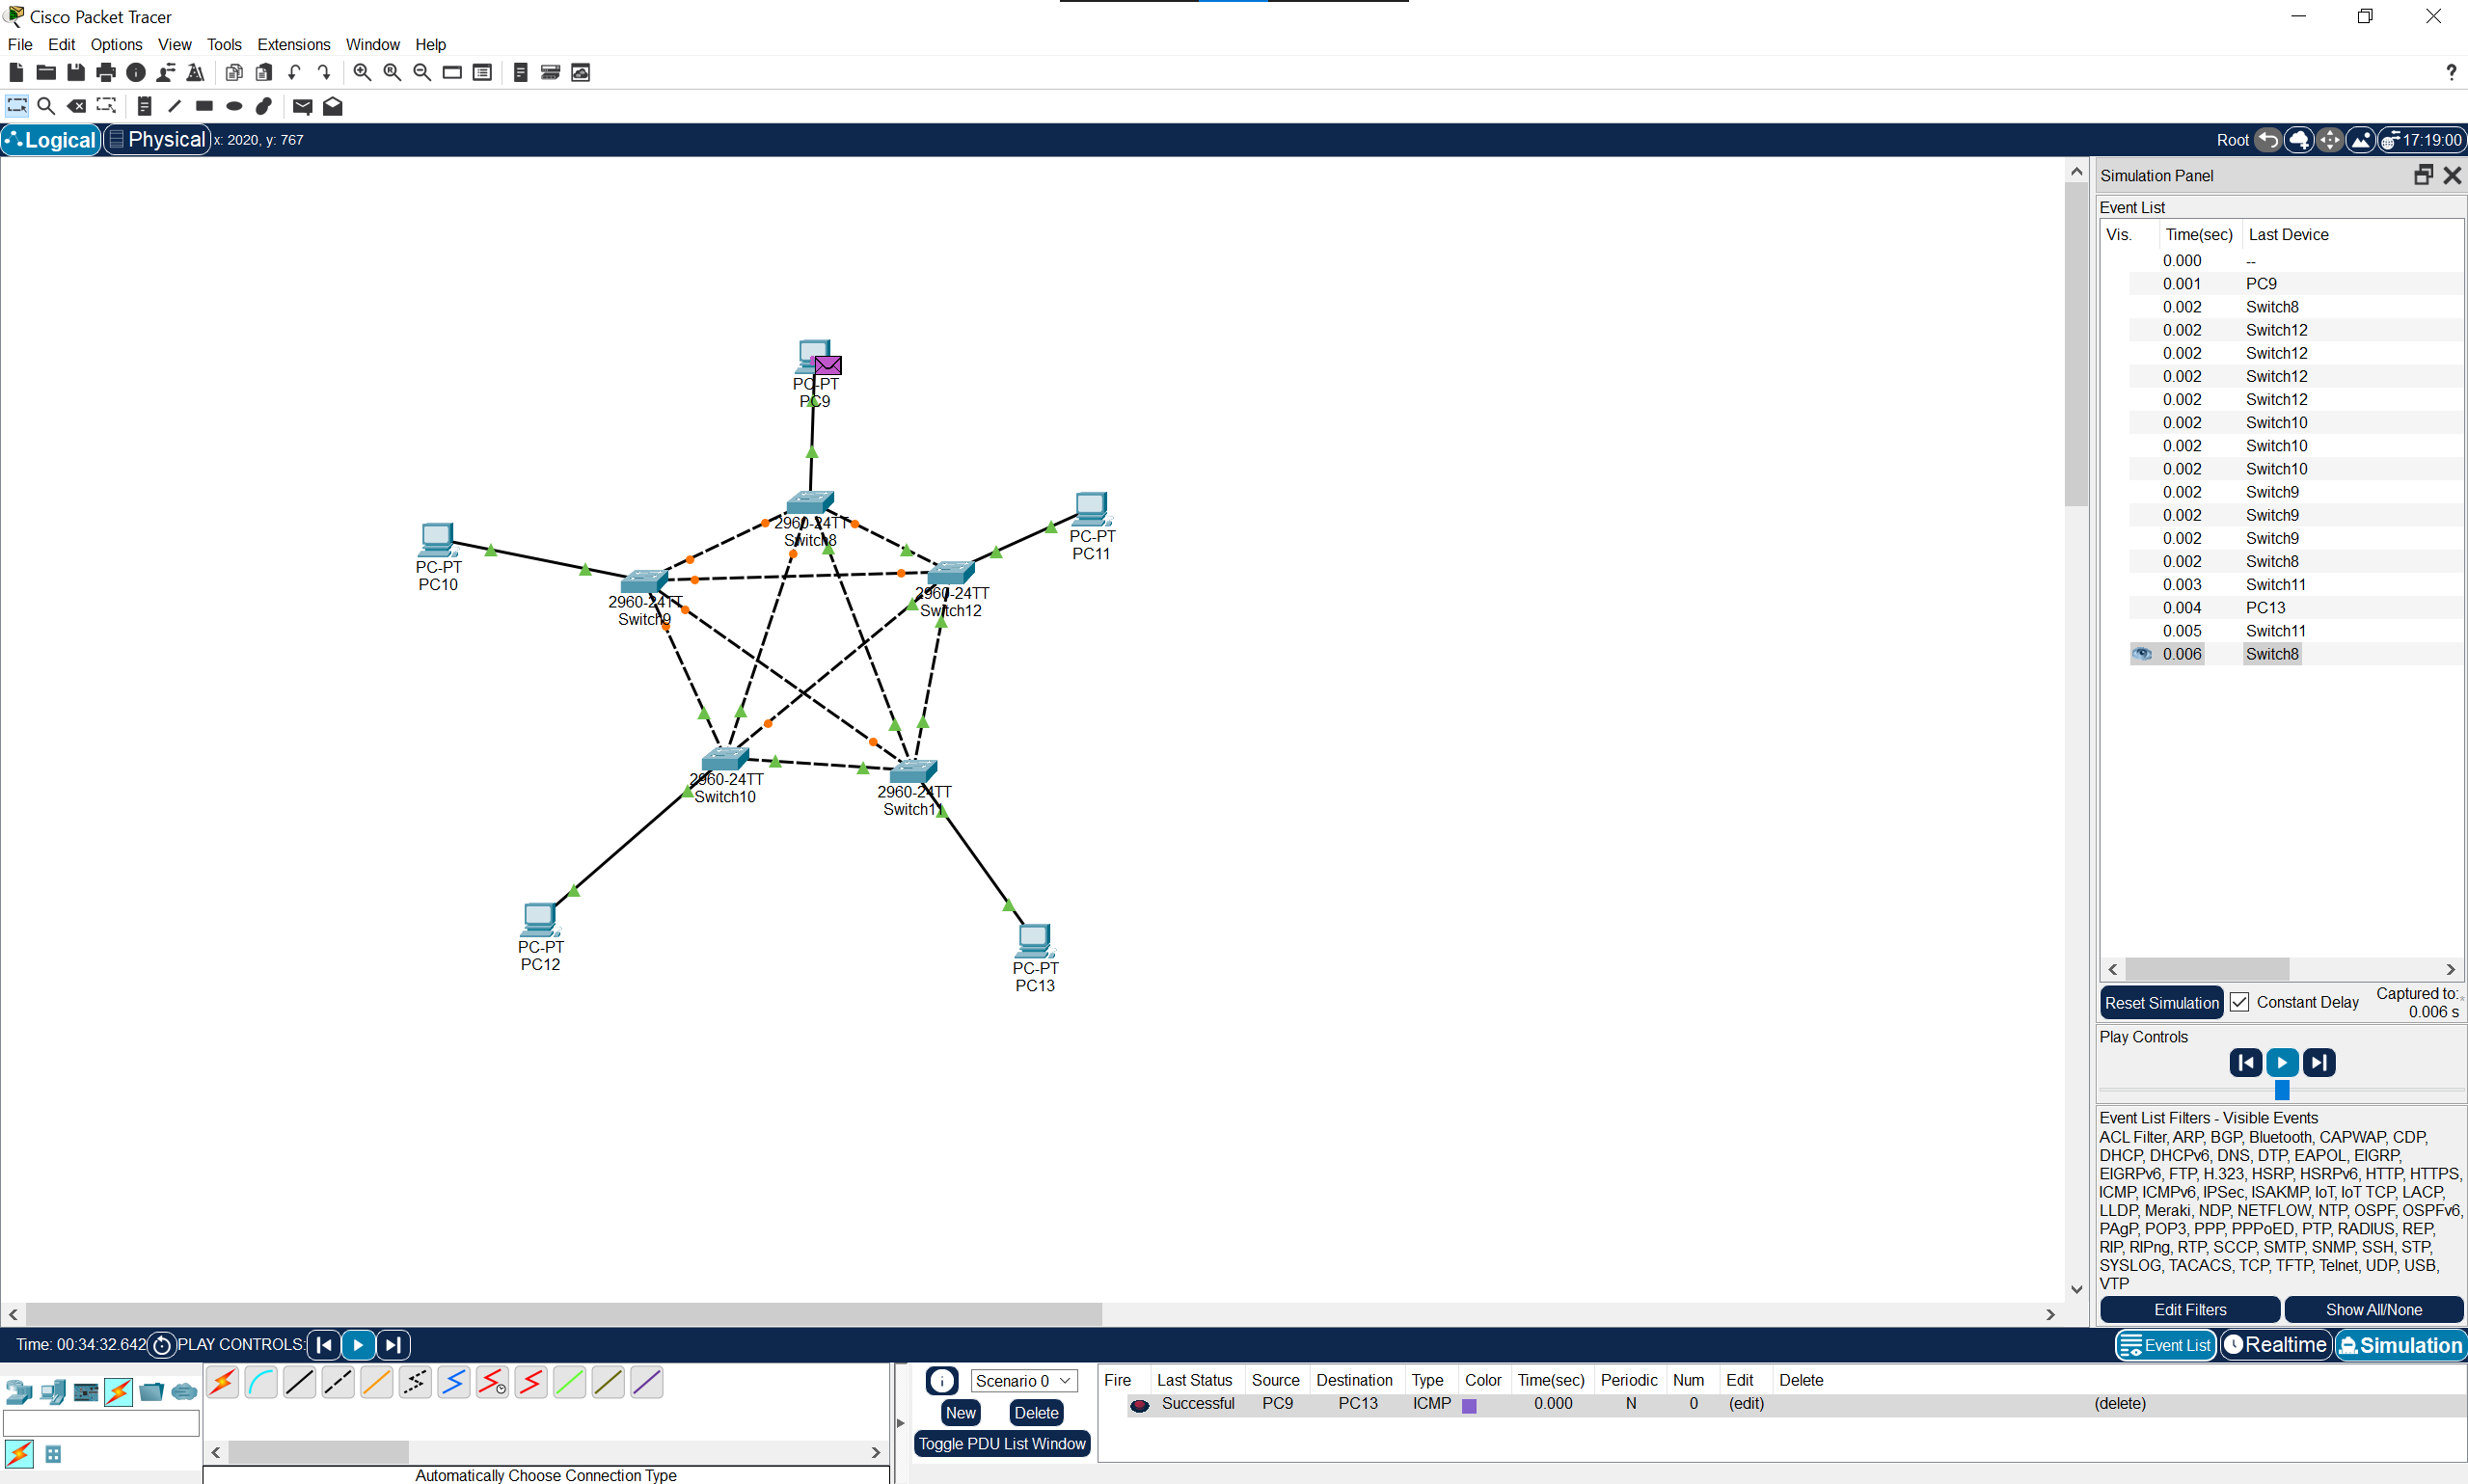
\includegraphics[width=\textwidth]{mesh.png}
\caption{Mesh topology}
\end{figure}
\end{document}
